\documentclass{beamer}
\mode<presentation>
{
  \usetheme{Warsaw}
  \definecolor{mcgarnet}{rgb}{0.38, 0, 0.08}
  \definecolor{mcgray}{rgb}{0.6, 0.6, 0.6}
  \setbeamercolor{structure}{fg=mcgarnet,bg=mcgray}
  %\setbeamercovered{transparent}
}

\usepackage[english]{babel}
\usepackage[latin1]{inputenc}
\usepackage{times}
\usepackage[T1]{fontenc}
\usepackage{tikz}
\usepackage{graphicx}

\newcommand{\imagesource}[1]{{\centering\hfill\break\hbox{\scriptsize Image Source:\thinspace{\small\itshape #1}}\par}}

\title{Backtracking}
\subtitle{\small Or How I Stopped Worrying and Learned to Love Brute Force}


\author{Robert Lowe\\}

\institute[Maryville College] % (optional, but mostly needed)
{
  Division of Mathematics and Computer Science\\
  Maryville College
}

\date[]{}
\subject{}

\pgfdeclareimage[height=0.5cm]{university-logo}{images/Maryville-College}
\logo{\pgfuseimage{university-logo}}



\AtBeginSection[]
{
  \begin{frame}<beamer>{Outline}
    \tableofcontents[currentsection]
  \end{frame}
}


\begin{document}

\begin{frame}
  \titlepage
\end{frame}

\begin{frame}{Outline}
  \tableofcontents
\end{frame}


% Structuring a talk is a difficult task and the following structure
% may not be suitable. Here are some rules that apply for this
% solution: 

% - Exactly two or three sections (other than the summary).
% - At *most* three subsections per section.
% - Talk about 30s to 2min per frame. So there should be between about
%   15 and 30 frames, all told.

% - A conference audience is likely to know very little of what you
%   are going to talk about. So *simplify*!
% - In a 20min talk, getting the main ideas across is hard
%   enough. Leave out details, even if it means being less precise than
%   you think necessary.
% - If you omit details that are vital to the proof/implementation,
%   just say so once. Everybody will be happy with that.

\section{The Backtracking Algorithm}
\begin{frame}
    \frametitle{Backtrackable Problems}
    \begin{columns}
        \column{0.5\textwidth}
        Problems where...
        \begin{itemize}[<+->]
            \item Correct solutions obey some set of constraints.
            \item Candidate solutions are enumerable.
            \item Candidate solutions are verifiable.
        \end{itemize}
        \column{0.5\textwidth}
        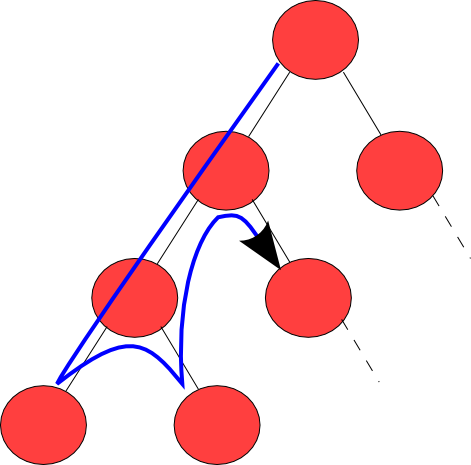
\includegraphics[width=\textwidth]{images/backtracking}
        \imagesource{wikipedia.org}
    \end{columns}
\end{frame}

\begin{frame}
    \frametitle{Brute Force Algorithms}
    \begin{columns}
    \column{0.5\textwidth}
    \begin{itemize}[<+->]
        \item Enumerate all possible sequences of moves.
        \item Choose one sequence that leads to a correct solution.
        \item Incredibly slow and expensive.
    \end{itemize}
    \column{0.5\textwidth}
    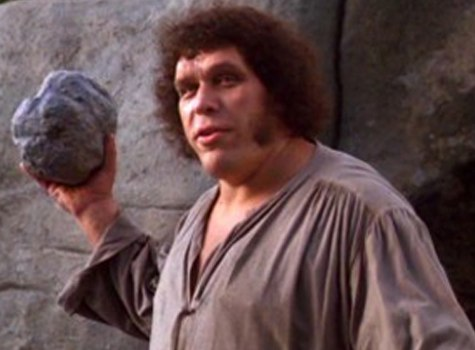
\includegraphics[width=\textwidth]{images/brute}
    \end{columns}
\end{frame}

\begin{frame}
    \frametitle{The Backtracking Algorithm}
    \begin{itemize}[<+->]
        \item Recursive algorithm which works by extending candidate solutions.
        \item Searches the space of possible solutions but prunes the search tree as it goes.
        \item Rejects solutions once there is no reason to continue expanding them.
        \item Much faster than pure brute force, though it can degenerate into a brute force condition.
    \end{itemize}
\end{frame}

\begin{frame}[fragile]
    \frametitle{A Generic Backtracking Class}
    \begin{verbatim}
class Candidate
{
public:
    //constructor
    Candidate();

    //returns true if this candidate is invalid or otherwise unworkable.
    virtual bool reject() = 0;
    
    //returns true if this candidate is a solved puzzle
    virtual bool solved() = 0;
    \end{verbatim}
\end{frame}

\begin{frame}[fragile]
    \frametitle{A Generic Backtracking Class (ctd.)}
\begin{verbatim}
    //returns the next extension of this candidate solution 
    //(nullptr if there is none)
    virtual Candidate *next() = 0;
   
    //carry out the backtracking algorithm and return a list of candidates
    //leading from this one to the finished solution
    virtual bool backtrack();

    //return the next step in the solution chain (if there is one)
    virtual Candidate *nextStep();

private:
    Candidate *_nextStep;
};
    \end{verbatim}
\end{frame}

\begin{frame}[fragile]
    \frametitle{The Backtracking Function}
    {\scriptsize
    \begin{verbatim}
bool Candidate::backtrack()
{
    //return an empty vector if we reject
    if(reject()) { return false; }
    
    //if we are solved, then this is the last step
    //in a solution chain
    if(solved()) { return true; }
    
    _nextStep = next();        //get the next candidate
    while(_nextStep != nullptr) {
        //backtrack from the next solution
        if(_nextStep->backtrack()) { return true; }
        
        //try again
        _nextStep = next();
    }
    
    return false;
}
\end{verbatim}
}
\end{frame}


\section{Back Tracking Problems}
\begin{frame}
    \frametitle{Sudoku Puzzles}
    \begin{columns}
        \column{0.5\textwidth}
        \begin{itemize}[<+->]
            \item Place the numbers 1-9 on 9x9 grid.
            \item No number can be repeated in a row.
            \item No number can be repeated in a column.
            \item No number can be created within the 9 3x3 grids.
        \end{itemize}
        \column{0.5\textwidth}
        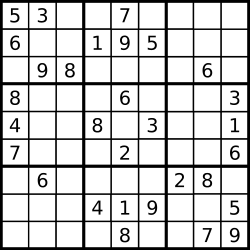
\includegraphics[width=\textwidth]{images/sudoku}
        \imagesource{wikipedia.org}
    \end{columns}
\end{frame}

\begin{frame}
    \frametitle{The N-Queens Problem}
    \begin{columns}
        \column{0.5\textwidth}
        \begin{itemize}[<+->]
            \item In Chess, a queen can move any number of spaces on 
              rank, file, or diagonal.
            \item Place n-queens on an nxn chess board so that no queen is attacking another queen.
        \end{itemize}
        \column{0.5\textwidth}
        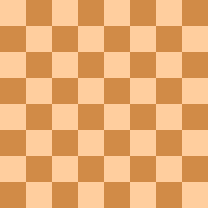
\includegraphics[width=\textwidth]{images/nqueens}
        \imagesource{wikipedia.org}
    \end{columns}
\end{frame}

\begin{frame}
    \frametitle{The Knight's Tour}
    \begin{columns}
        \column{0.5\textwidth}
        \begin{itemize}[<+->]
            \item A knight can move to a square that is either 2 squares horizontally and 1 vertically away or to one that is 1 square horizontally and 2 vertically away.
            \item Place a knight at an arbitrary position on the chess board.
            \item Using only legal knight moves, land on each square on the board exactly one time.
        \end{itemize}
        \column{0.5\textwidth}
        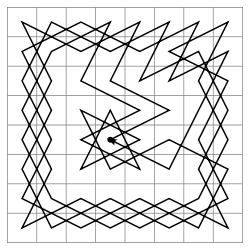
\includegraphics[width=\textwidth]{images/knights}
        \imagesource{wikipedia.org}
    \end{columns}
\end{frame}

\end{document}


